\documentclass[letterpaper]{article}

\usepackage{amssymb}
\usepackage{amsthm}
\usepackage{amsmath}
\usepackage[left=1in, right=1in, top=1in, bottom=1in]{geometry}
\usepackage{graphicx}

\newcommand{\ZZ}{\mathbb{Z}}
\newcommand{\NN}{\mathbb{N}}
\newcommand{\QQ}{\mathbb{Q}}

\newtheorem{lemma}{Lemma}
\newtheorem{sublemma}{Lemma}[lemma]
\newtheorem{theorem}{Theorem}[section]
\newtheorem{corollary}{Corollary}[section]
\newtheorem{definition}{Definition}[section]
\newtheorem{proposition}{Proposition}[section]
\newtheorem{example}{Example}[theorem]

\title{M 328K: Lecture 7}
\author{Katherine Ho}
\date\today

\begin{document}
\maketitle

\section{Last Time}
\begin{enumerate}
    \item $ax\equiv b \pmod{n}$
        If $d=\gcd(a,n)$, then 
        \begin{enumerate}
            \item If $d\nmid b$, then no solutions
            \item If $d\mid b$, then there are exsactly $d$ distinct solutions mod $n$
            \item If $\gcd(a,n)=1$, there is a unique solution mod $n$.
        \end{enumerate}
    \item $9x\equiv 21 \pmod{30}$ \\
        $d=\gcd(9,30)=3$ \\
        First divide by $d$ to solve congruence
        \[ 3x\equiv 7\pmod{10} \] 
        This applies to point 1(c) and has a \underline{unique} solution mod 10. \\
        Euclidean Algorithm: $x=-21$ is a solution.  There are infinitely many solutions
        adding multiples of 10 to the solution.
        \[ -21+10k \quad\text{is also a solution} \]
        They are all congruent to each other mod 10.
        Infinitely many integer solutions to $3x\equiv 7\pmod{10}$ are
        \[ \dots,-21,-11,-1,9,19,29,39,\dots \]
        This list \underline{also} includes all solutions to original congruence, 
        \underline{but} not all the same mod 30.
\end{enumerate}
    
\section{Today}
    Consider $ax\equiv 1\pmod{n}$. This has a (unique) solution iff 
    $\gcd(a,n)=1$. \\
    A solution is called a \underline{multiplicative inverse of
    a modulo n}. We will write it as $x\equiv a^{-1}\pmod{n}$ so $aa^{-1}\equiv 1\pmod{n}$.
    Note that $a^{-1}\ne \frac{1}{a}$. \\
    \underline{Recall}. $4x\equiv 3\pmod{19}$. \\
    Note. 
    \begin{align*}
        4^{-1} &\equiv 3\pmod{19} \quad\text{Since} \\
        4\cdot 5 &\equiv 20\equiv 1\pmod{19}
    \end{align*}
    Multiply $4x\equiv 3\pmod{19}$ by $4^{-1}\pmod{19}$ to get 
    \begin{align*}
        5\cdot 4x &\equiv 5\cdot 3\pmod{19} \\
        x &\equiv 15 \pmod{19}
    \end{align*} 

    \begin{example}
        Find $7^{-1}\pmod{17}$. 
        Solve $7x\equiv 1\pmod{17} \Leftrightarrow 7x-17y=1$. \\
        EA:
        \begin{align*}
            17 &= 7\cdot 2 + 3 \\
            7 &= 3\cdot 2 + 1 \\
            1 &= 7-3\cdot 2 \\ 
            1 &= 7-(17-7\cdot 2) \\
            &= 17(-2)+7\cdot 5
        \end{align*}
        \begin{center}\boxed{$x = 5$}\end{center}
    \end{example}

\section{Stuff}
    $a^k\pmod{5}$  \\
    \begin{center}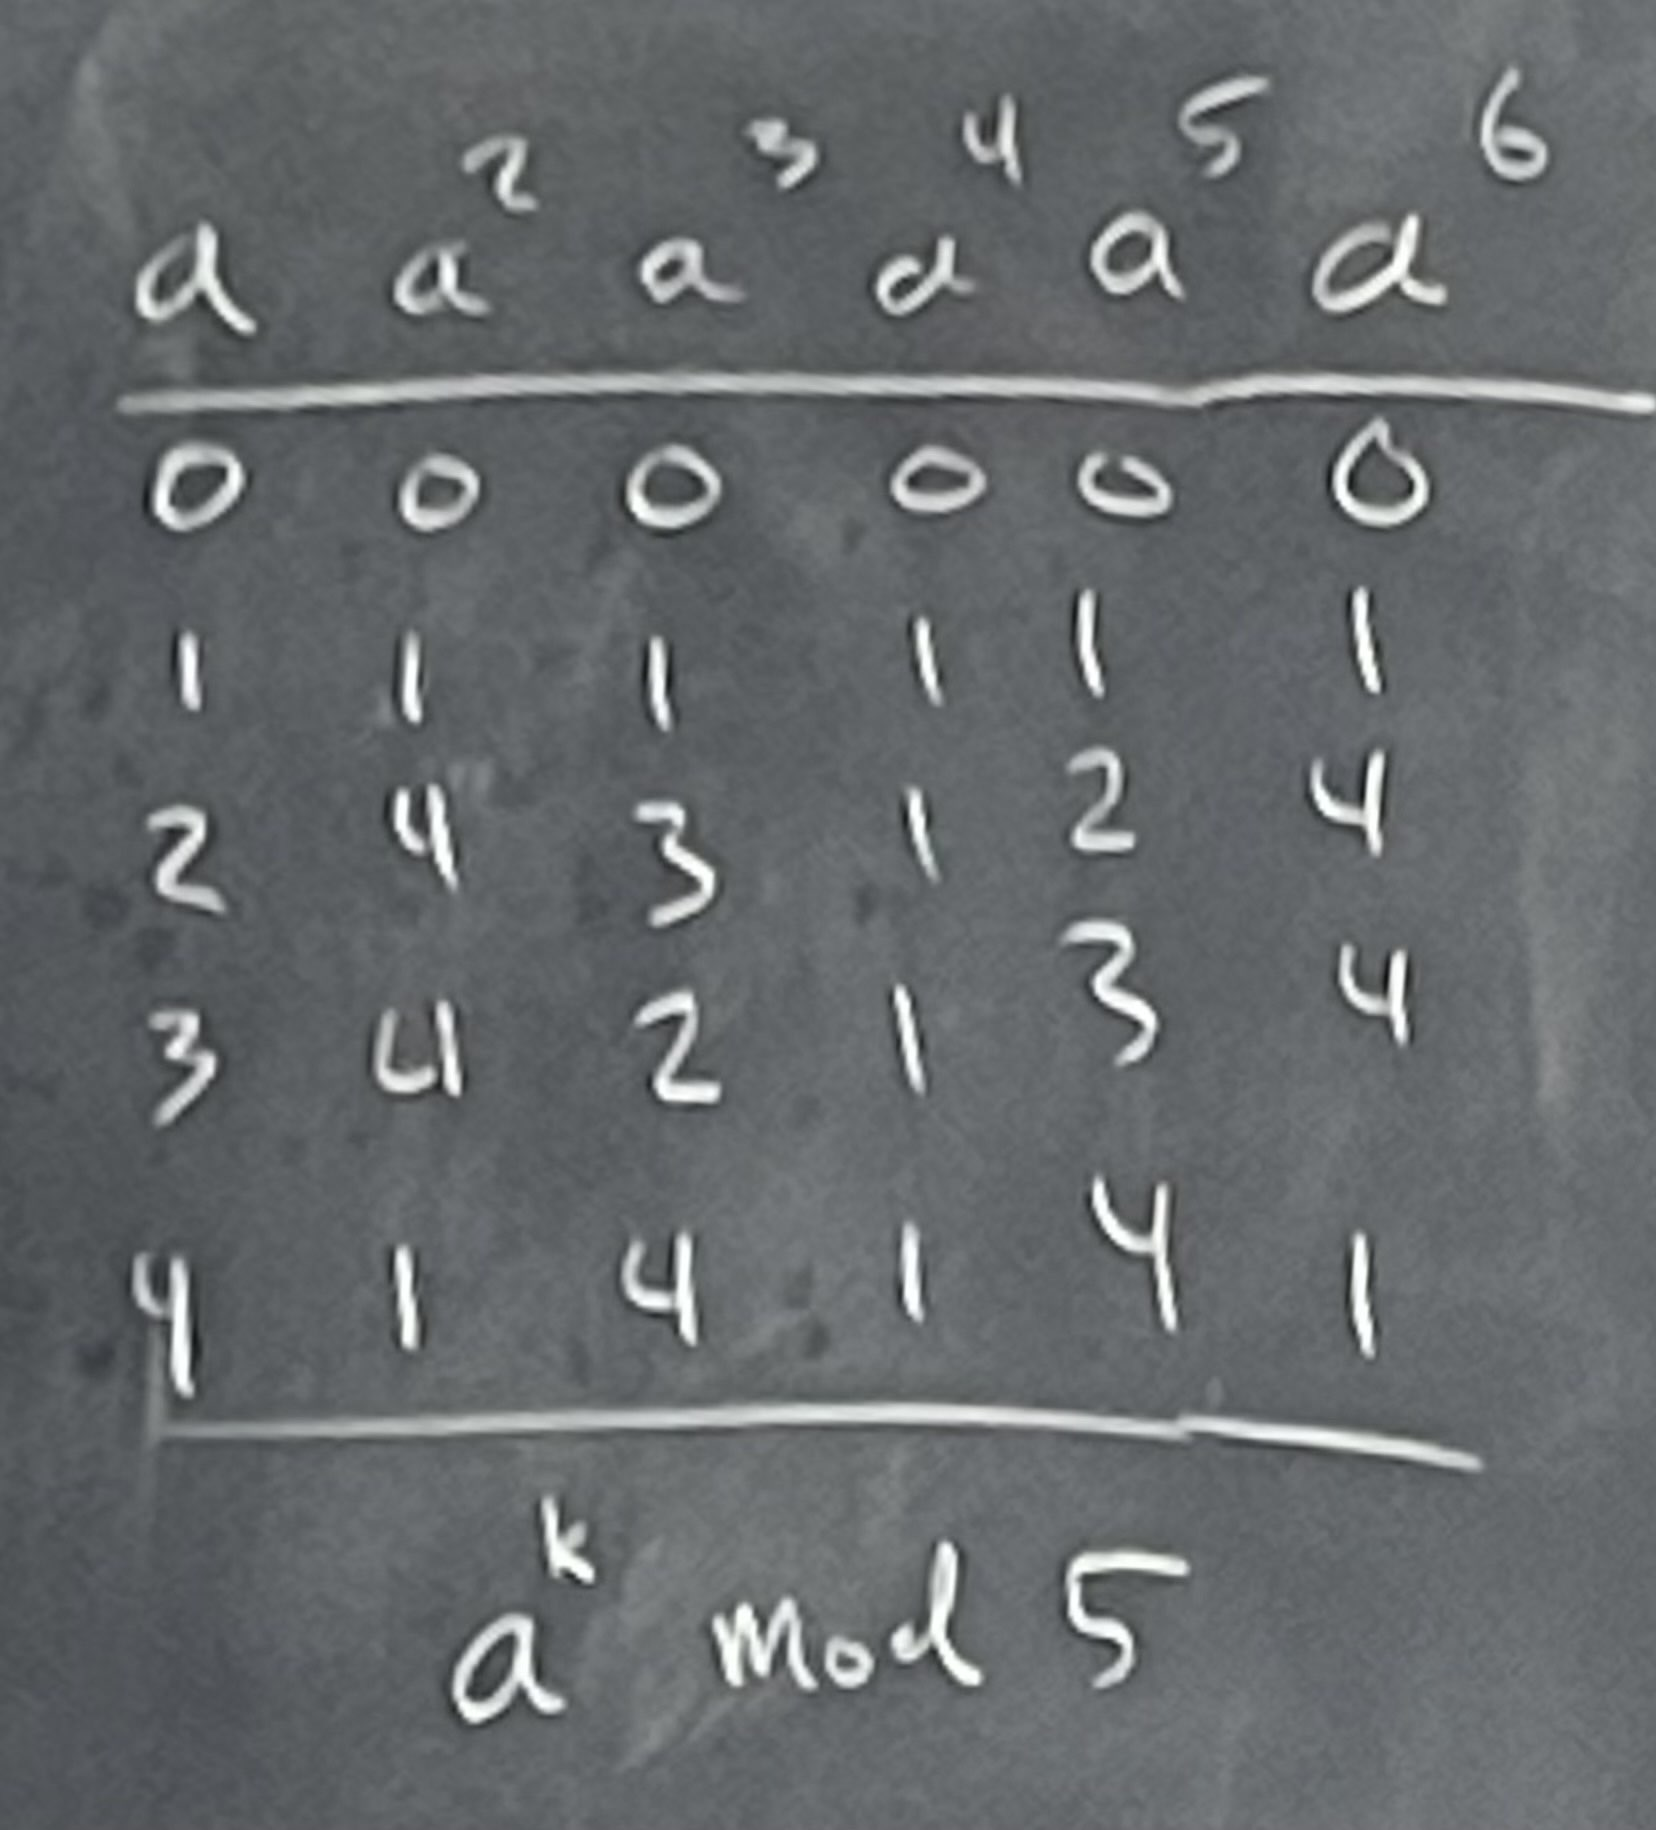
\includegraphics[scale=0.1]{image1.jpg}\end{center}
    $a^k\pmod{7}$ \\
    \begin{center}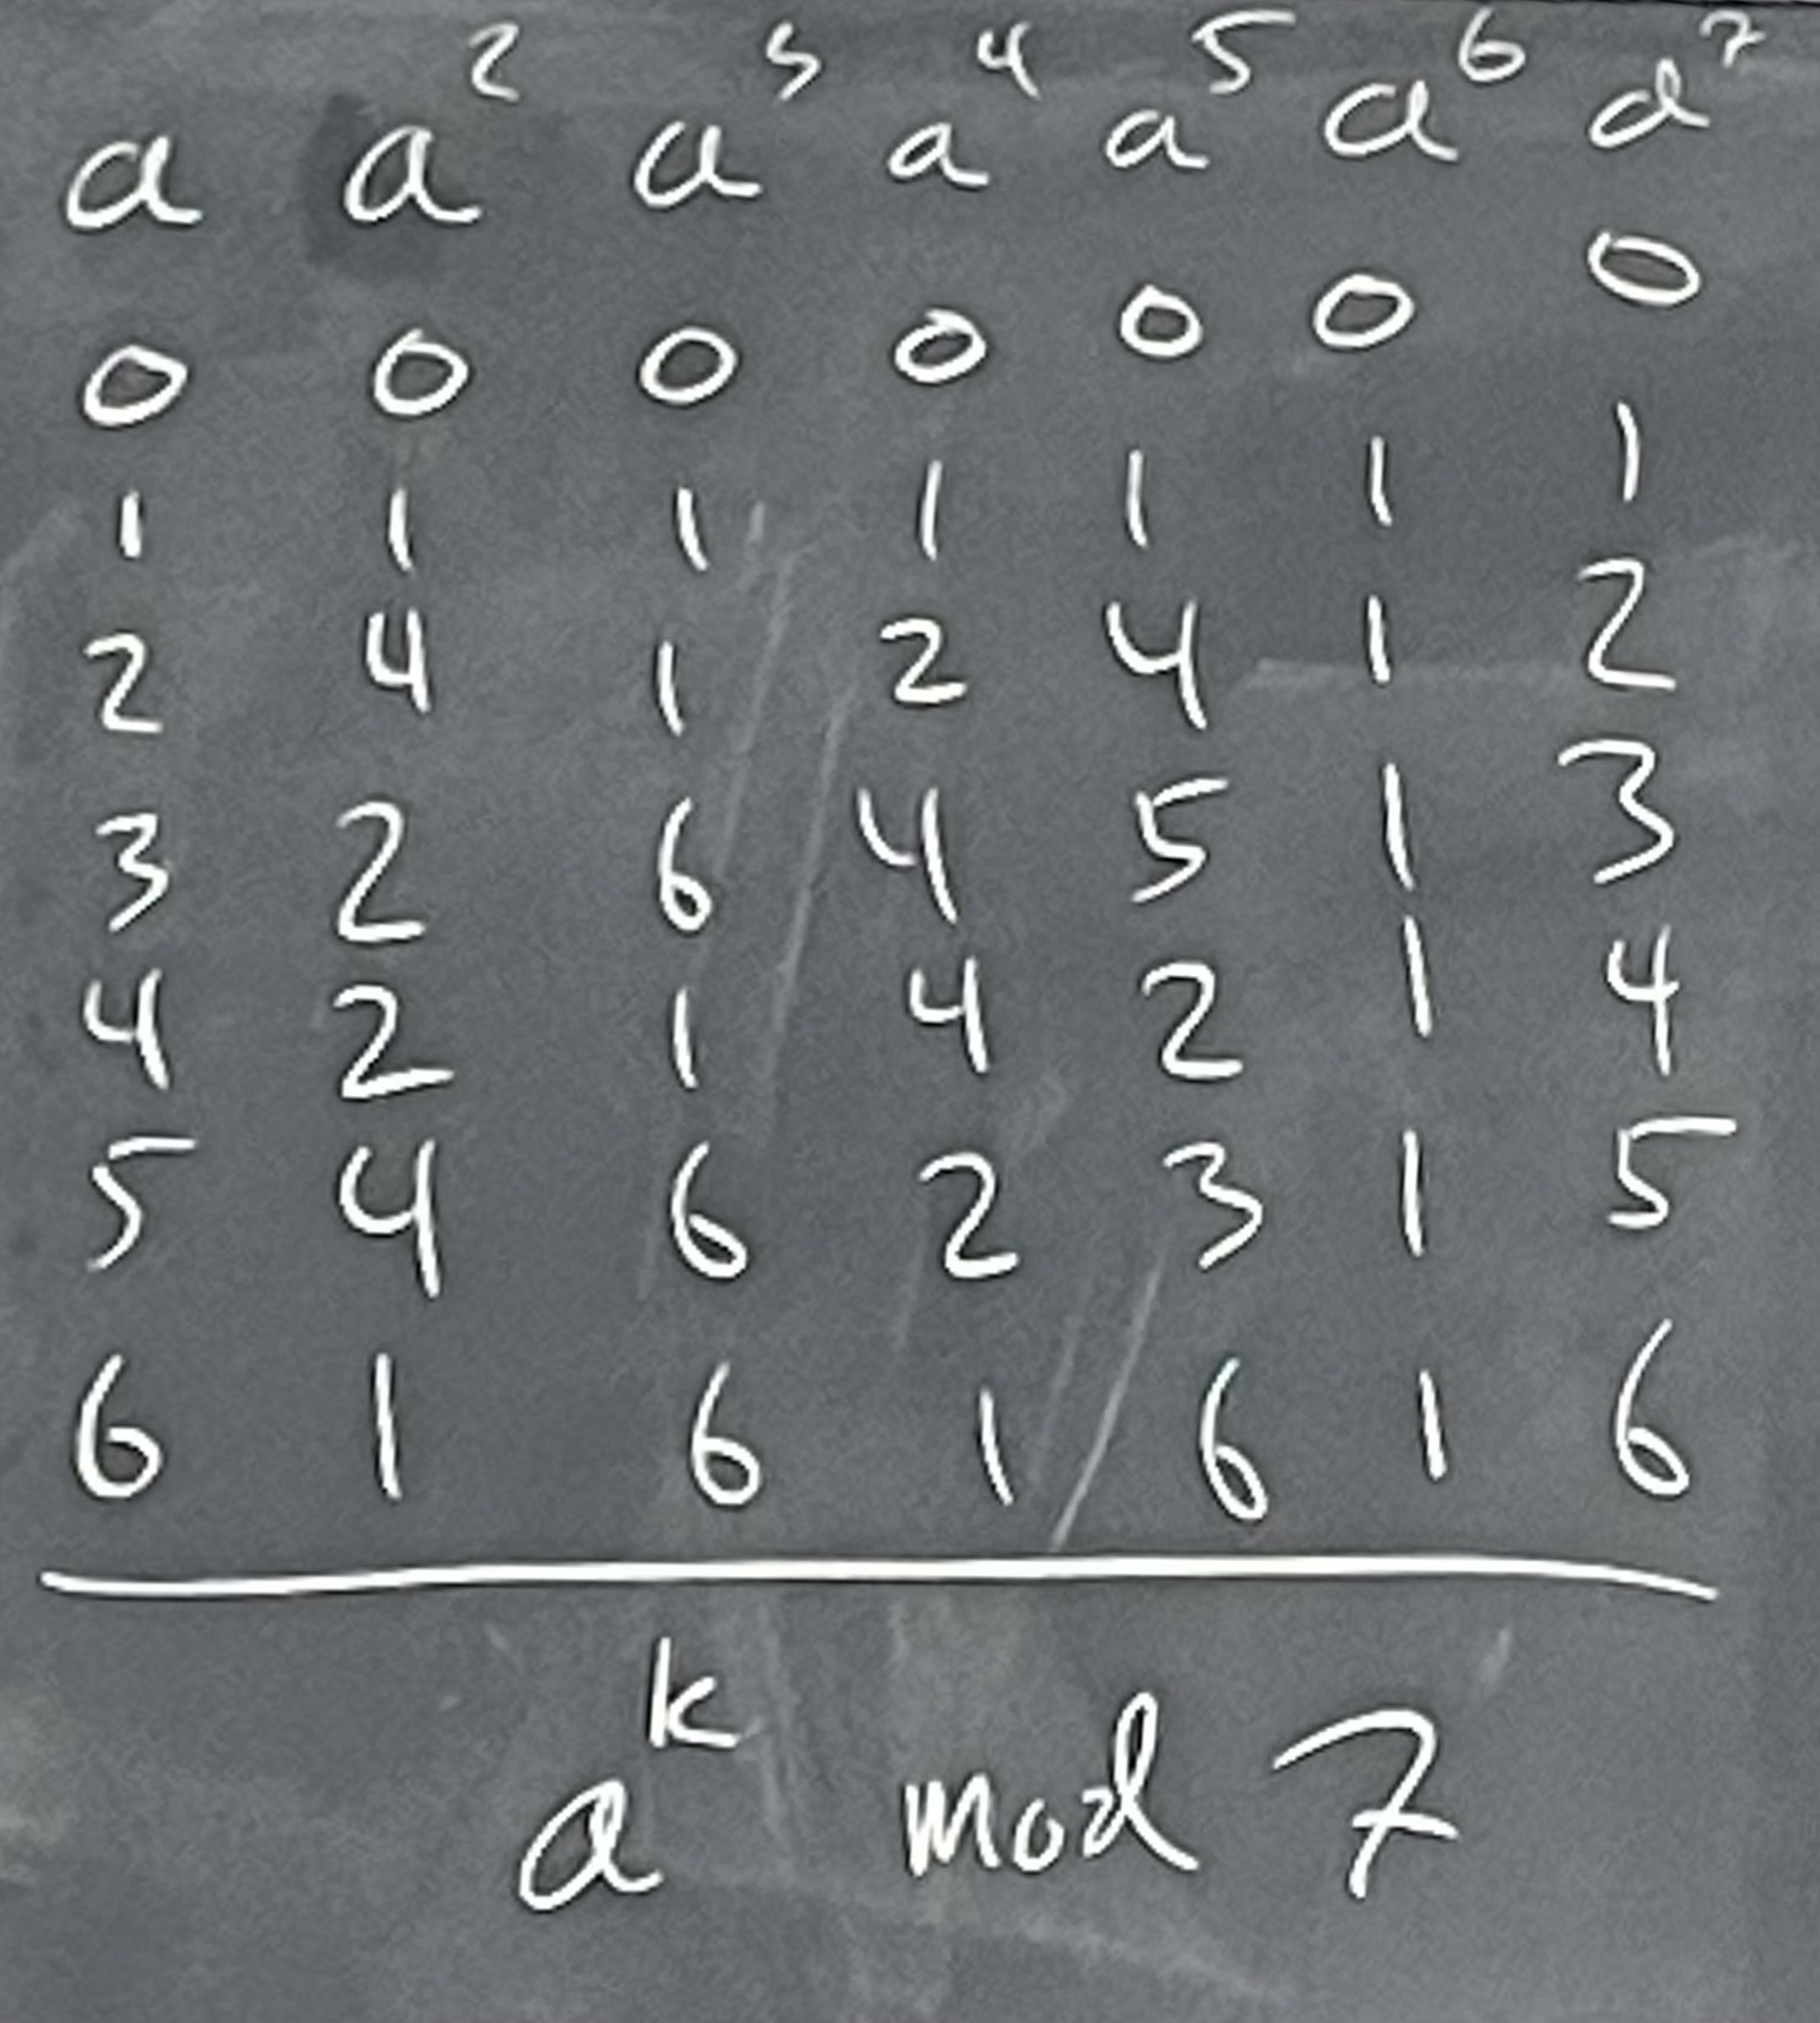
\includegraphics[scale=0.08]{image2.jpg}\end{center}

    \subsection{Fermat's Little Theorem}
        \begin{theorem}
            Let $p$ be prime and $a\in\ZZ$ such that $p\nmid a$. Then
            \[
                a^{p-1}\equiv 1\pmod{p}
            \]
            ie.
            \[ 
                p\mid (a^{p-1}-1)
            \]
        \end{theorem}

        \begin{proof} [Proof (Idea)]
            $p=5$ 
            \begin{align*}
                0,1,2,3,4,5 \pmod{5} \\
                0,2,4,1,3 \pmod{5} \\
                0,3,1,4,2
            \end{align*}
        \end{proof}

        \underline{Claim}: The integers $0,a,2a,\dots, (p-1)a \pmod{p}$
        are the same as the integers $0,1,2,\dots,(p-1)$ but maybe
        in a different order.

        \begin{proof} [Proof of Claim]
            If claim is false, then $ia\equiv ja\pmod{p}$ for some $i,j$. 
            Then $p\mid a(i-j)$. \\
        \end{proof}

        Now Consider
        \begin{align*}
            & a(2a)(3a)\dots((p-1)(a)) \\
            &= a^{p-1}(1)(2)(3)\dots(p-1) \\
            &= a^{p-1}(p-1)!
        \end{align*}
        On the other hand, by the claim, 
        \begin{align*}
            a(2a)(3a)\dots((p-1)a) &\equiv (1)(2)(3)\dots(p-1) \pmod{p} \\
            a^{p-1}(p-1)! &\equiv (p-1)! \pmod{p}
        \end{align*}
        By HW, 
        \[ \gcd((p-1)!, p) = 1 \]
        So we can cancel: 
        \[ a^{p-1}\equiv 1\pmod{p} \]
        
    \subsection{Example}
            $p=23$. $6^{22}=1\pmod{23}$.  \\
            ie. \[ 23|(6^{22}-1) \]
        
    \subsection{Primality Test}
    $n=10^{100}+37$ \\
    Compute 
    \begin{align*} 
        2^{n-1} = 2^{10^{100}+36}\not\equiv 1\pmod{n} \\
        \equiv 367\dots 396\pmod{n}
    \end{align*}
    So n is \underline{not prime}. \\
    Note: This will \underline{never} show n is prime. It can be true that $a^{n-1}\equiv 1\pmod{n}$
    even if n is composite. \\
    Test 117 with $a=2$. 
    \begin{align*}
        2^{116} &= 2^{64}\cdot 2^{32}\cdot 2^{16}\cdot 2^{4} \\
        &\equiv 16\cdot 22 \cdot 16 \cdot 16 \\
        &\equiv 22 \\
        &\not\equiv 1\pmod{117}
    \end{align*}
    So 117 is composite.     

\end{document}